\documentclass{article}
% --- watermark (auto-inserted) ---
\usepackage{xcolor}
\usepackage{xfp}% \fpeval; in the kernel since 2022, harmless on older LaTeX
\usepackage{draftwatermark}
\newlength{\watermarkTextWidth}
\AddToHook{begindocument/end}{%
  \SetWatermarkText{\normalfont Generated by The Agentic Scientist}%
  \SetWatermarkFontSize{10pt}%
  \SetWatermarkLightness{0.85}%
  \settowidth{\watermarkTextWidth}{\normalfont\fontsize{10pt}{12pt}\selectfont Generated by The Agentic Scientist}%
  \edef\watermarkScale{\fpeval{0.8 * sqrt(\paperwidth**2 + \paperheight**2) / \watermarkTextWidth}}%
  \edef\watermarkAngle{\fpeval{atand(\paperheight/\paperwidth)}}%
  \SetWatermarkScale{\watermarkScale}%
  \SetWatermarkAngle{\watermarkAngle}%
}
% --- end watermark ---
\usepackage{paper,times}
\usepackage{amsmath,amssymb,booktabs,longtable,array,graphicx,subcaption}
\usepackage{hyperref,url}
\title{Adaptive ILR Ellipsoids: Coverage--Volume Trade-offs on the Simplex}
\author{Anonymous authors}
\newcommand{\simplex}{\Delta^{K-1}_{+}}
\newcommand{\R}{\mathbb{R}}
\newcommand{\clip}{\operatorname{clip}}
\begin{document}
\maketitle

\begin{abstract}
Prediction regions for continuous compositions must be evaluated both for joint coverage and for their size on the simplex. We study whether training-adaptive isometric log-ratio (ILR) ellipsoids offer a useful coverage--volume trade-off relative to Euclidean and isotropic ILR balls. The adaptive configuration estimates residual scales and boundary-dependent shapes using training data, while an independent split-conformal calibration determines the region threshold. Across five held-out seeds and six synthetic conditions, heteroskedastic logistic-normal responses yield mean coverage 0.9044 and simplex-volume fraction 0.1476, compared with 0.9030 and 0.3336 for Euclidean balls. The benefit is not uniform: boundary-concentrated Dirichlet responses require volume fraction 0.9759, while covariate-shifted coverage falls to 0.8633 against a 0.90 target. Descriptive sign-stratum coverage also remains uneven. These findings support condition-dependent evaluation of region geometry, not universal superiority or conditional validity. Common-measure integration and separate uncertainty summaries expose failures that a single aggregate objective would obscure.
% @evidence[[paper_data.json#final_evaluation.evaluation_evidence.episodes]]
% @evidence[[derived/summary.json]]
\end{abstract}

\section{Introduction}
Compositional responses describe how a whole is distributed among its parts: each component is nonnegative and the components sum to one. Uncertainty about an observed composition is therefore a joint, constrained prediction problem. An interval for every component does not by itself specify a calibrated joint region, and a region that covers almost the entire simplex can be reliable yet uninformative. This distinction matters even when the point predictor is accurate. We consider continuous composition-valued responses, not the discrete label of a classifier or an unobserved population probability vector.

Conformal prediction separates the quality of a fitted predictor from the calibration of its prediction region \citep{Vovk2005,Papadopoulos2002,Angelopoulos2021}. Under exchangeability, a calibration sample supplies a finite-sample marginal coverage guarantee for a frozen score. That guarantee does not choose the score geometry, ensure small regions, or establish coverage at particular covariate values. Compositional geometry introduces an additional choice: distances in raw proportion coordinates and distances in log-ratio coordinates need not describe similarly sized subsets of the simplex \citep{Aitchison1982,Egozcue2003}. Comparing calibrated radii across these spaces is consequently insufficient.

Our question is whether a training-adaptive ILR residual geometry yields smaller prediction regions at comparable observed joint coverage, and which conditions defeat that trade-off. We study a specific configuration that combines held-out training residuals, covariate-dependent diagonal scales, and training-defined boundary groups. Its threshold is calibrated independently, using the same split-conformal rule as two simpler reference geometries. All regions are evaluated by membership and by the same normalized simplex-volume measure. This makes the comparison meaningful even when their native coordinate systems differ.

The empirical contribution is deliberately scoped. We provide a matched evaluation of the three region families across homoskedastic, heteroskedastic, boundary-concentrated, and shifted synthetic responses, together with information-removal controls. We expose the distinction between integration error, finite-test uncertainty, and between-seed dispersion. We also retain a direct comparison of alternative adaptive training configurations, while explicitly declining to attribute bundled changes to cross-fitting alone. The central finding is a useful heteroskedastic trade-off accompanied by substantial boundary inefficiency and persistent shifted undercoverage; it is not a new universal conformal guarantee.
% @evidence[[paper_data.json#final_evaluation.evaluation_evidence.episodes]]
% @evidence[[source_evidence/adaptive.py#L90-L131]]

\begin{figure}[t]
\centering

\includegraphics[width=\textwidth]{figures/geometry_calibration_overview.png}
\caption{Study overview. Training data determine the location and geometry; independent calibration determines a single threshold. Euclidean balls, ILR balls, and adaptive ILR ellipsoids are compared by joint response coverage and a common simplex-volume measure. Boundary groups adapt shape, not calibration. Any simplex icon is conceptual, not a measured response cloud.}
\label{fig:overview}
\end{figure}

\section{Related Work}
\paragraph{Composition-valued prediction.}
Logistic-normal models describe continuous distributions on the simplex through transformed Gaussian coordinates \citep{AitchisonShen1980}. Log-ratio analysis addresses the dependence imposed by closure; ILR coordinates provide an orthonormal representation of its contrast space \citep{Aitchison1982,Egozcue2003,Pawlowsky2011}. We use this representation as a working geometry, not as evidence that all simplex distributions become well approximated by ellipsoids. In particular, strictly positive Dirichlet responses can lie close to the boundary, where log ratios are highly sensitive to small components.

\paragraph{Calibration and adaptation.}
Split-conformal regression permits flexible fitted scores with marginal calibration \citep{Lei2018}; conformalized quantile regression adapts scalar intervals to heteroskedasticity \citep{Romano2019}. For joint multivariate responses, \citet{Henderson2024} construct ellipsoids using covariate--residual Mahalanobis scores, exchangeability-preserving covariance estimation, and covariate-dependent centers and radii. Here, residual rescaling occurs in ILR coordinates with training-frozen geometry and independent scalar calibration. We do not evaluate their method or transfer its volume comparisons to the simplex. Cross-validation and predictive sample reuse motivate held-out residual estimation \citep{Stone1974,Geisser1975}, but residual cross-fitting is not conformal calibration. Unlike jackknife+, which combines leave-one-out predictions and residuals \citep{Barber2021Jackknife}, our construction requires a separate calibration sample.
% @evidence[[literature/Henderson2024/reading.json]]
% @evidence[[literature/Henderson2024/method_excerpt.txt]]

\paragraph{Coverage targets and evaluation.}
Conditional validity is stronger than marginal validity, and distribution-free conditional inference faces fundamental limitations \citep{Vovk2012,Barber2021Limits}. Label-adaptive and class-conditional classification methods address distinct targets from coverage of an observed continuous composition \citep{Romano2020,Ding2023}. Weighted conformal methods and extensions beyond exchangeability address distribution shift with additional structure \citep{Tibshirani2019,Barber2023}; we do not implement those corrections. Instead, shift is an explicit stress test. Finally, our coverage--volume objective is not a proper scoring rule for a predictive distribution \citep{Gneiting2007}. Reporting its components separately is necessary to distinguish empirical compactness from reliability.

\section{Method}
\subsection{Problem Setup and Design Rationale}
Let $X\in\R^5$ and $Y\in\simplex=\{y\in(0,1)^K:\sum_j y_j=1\}$. The target is a region $C_\alpha(X)$ containing a future observed composition with probability at least $1-\alpha$, marginally under an exchangeable calibration/test law. The evaluated target is $\alpha=0.1$. We study joint membership of the entire response vector; neither componentwise intervals nor coverage of a latent distribution is the estimand. The empirical trade-off is test coverage versus normalized volume under the uniform distribution on the simplex.
% @evidence[[source_evidence/evaluate_final.py#L34-L45]]
% @evidence[[paper_data.json#final_evaluation.evaluation_evidence.episodes]]

The working hypothesis is that a pooled residual norm wastes volume when residual scales vary predictably with $X$. Training-derived scale and shape adjustments may align the region with this heterogeneity before calibration. Boundary-dependent shapes are a limited proxy for variation in residual geometry, not a guarantee of local validity. The countervailing hypothesis is that log-ratio tail behavior or covariate shift can defeat compactness or coverage despite this adaptation. These hypotheses concern end-to-end configurations: the experiment does not isolate the causal contribution of every fitted component.

\subsection{Reference Geometries}
Choose $B\in\R^{K\times(K-1)}$ with $B^TB=I$ and $B^T\mathbf{1}=0$. Write $z(y)=B^T\log y$ and $h(z)=\operatorname{softmax}(Bz)$. All location models use a quadratic design $\phi(x)$ containing an intercept, each input, its square, and distinct pairwise products. Ridge fits use penalty $0.01$, including the intercept \citep{HoerlKennard1970}. The Euclidean reference fits responses directly, clips fitted components below $10^{-12}$, renormalizes, and uses $s_E(x,y)=\|y-\widehat p(x)\|_2$. The ILR reference fits $z(Y)$ and uses $s_I(x,y)=\|z(y)-\widehat m_I(x)\|_2$. Both references fit locations on the first three quarters of the available training rows. Their calibrated sets are respectively simplex-intersected Euclidean balls and inverse-ILR images of isotropic balls.
% @evidence[[source_evidence/evaluate_final.py#L624-L680]]

\subsection{Training-Adaptive ILR Residual Geometry}
The studied adaptive configuration partitions training rows deterministically into four folds by row index modulo four. Each row receives a residual $r_i=z(y_i)-\widehat m^{(-f(i))}(x_i)$ from a ridge location fit excluding its fold. A final location $\widehat m$ is refitted on all training rows. For each ILR coordinate, a second ridge regression with penalty $5$ fits $\log(r_{ij}^2+0.02)$ on $\phi(x_i)$. With fitted value $v_j(x)$, define
\begin{equation}
 D(x)=\operatorname{diag}(\sigma_j(x)),\qquad
 \sigma_j(x)=\exp\!\left\{\tfrac12\clip(v_j(x),-6,5)\right\}.
 \label{eq:scale}
\end{equation}
The standardized residual vector $u_i=D(x_i)^{-1}r_i$ is clipped coordinatewise to $[-1000,1000]$. These safeguards are fixed numerical choices, not independently optimized or ablated findings.
% @evidence[[source_evidence/adaptive.py#L90-L123]]

Boundary proximity is summarized by $b(x)=\min_j h(\widehat m(x))_j$. Training predictions define its lower and upper tertiles; right-sided threshold assignment gives a group $g(x)$. For dimension $d=K-1$, the fitted second-moment shapes are
\begin{equation}
 S_0=\frac{\sum_i u_i u_i^T+8I_d}{n_{\rm tr}+8},\qquad
 S_g=\frac{\sum_{i:g(x_i)=g}u_i u_i^T+32S_0}{n_g+32}.
 \label{eq:shape}
\end{equation}
Let $H_gH_g^T=S_g$ be its Cholesky factor and $L(x)=D(x)H_{g(x)}$. The adaptive score is
\begin{equation}
 s_A(x,y)=\left\|L(x)^{-1}\{z(y)-\widehat m(x)\}\right\|_2.
 \label{eq:score}
\end{equation}
These are uncentered residual second moments, not unbiased sample covariances. Shrinkage toward a positive target stabilizes the shapes, in the broad spirit of covariance regularization \citep{SchaferStrimmer2005,Chen2010}; this is not an implementation of either cited estimator. All group boundaries, scales, and factors are frozen before calibration. Only the residual geometry is group-dependent: no groupwise conformal quantiles are fitted.
% @evidence[[source_evidence/adaptive.py#L116-L131]]
% @evidence[[source_evidence/adaptive.py#L190-L198]]

\subsection{Independent Calibration and Guarantee Scope}
For any one of the frozen scores, sort its $n_{\rm cal}$ calibration values and select rank $k=\lceil(n_{\rm cal}+1)(1-\alpha)\rceil$. Use $q=+\infty$ if $k>n_{\rm cal}$; otherwise use the $k$th value. The region is $C_\alpha(x)=\{y\in\simplex:s(x,y)\le q\}$. Conditional on a fixed training fit, exchangeability of the calibration and future scores gives the standard rank argument:
\begin{equation}
 \Pr\{Y_{\rm new}\in C_\alpha(X_{\rm new})\}\ge 1-\alpha.
 \label{eq:coverage}
\end{equation}
With no ties the rank is uniform among the calibration-plus-test scores; ties with the nonrandomized inclusion rule make the bound conservative. This is the usual split-conformal argument \citep{Lei2018,Angelopoulos2021}, not a new theorem. It does not lower-bound every realized finite-test coverage fraction, require Gaussian residuals, or establish conditional coverage. Under test-only covariate shift the exchangeability premise fails. Training cross-fitting can affect efficiency, but does not repair that premise.
% @evidence[[source_evidence/evaluate_final.py#L859-L864]]

\section{Experimental Protocol}
\subsection{Synthetic Conditions and Comparators}
The released study covers a single composition-regression task, with $K=3$ or $8$ and five Gaussian covariates. Four response conditions are paired with two information-removal controls. The homoskedastic condition (C1) uses a quadratic ILR mean and Gaussian noise with scale $0.35$. The heteroskedastic condition (C2) multiplies that scale by $\exp\{0.65\clip(x_1,-3,3)\}$ and coordinate-specific factors from $0.5$ to $1.5$. These two conditions have $K=3$. The boundary condition (C3) has $K=8$ and uses a Dirichlet response with a shifted ILR mean and low concentrations. The shifted condition (C4), also with $K=8$, uses a different Dirichlet concentration and modifies test covariates only: $x_1$ increases by $1.5$ and $x_2$ is multiplied by $1.5$. Appendix~\ref{sec:generators} gives the precise generator. All responses are strictly positive; structural zeros are not evaluated.
% @evidence[[source_evidence/evaluate_final.py#L776-L814]]
% @evidence[[source_evidence/final_resource_manifest.json]]

The constant-input control (C5) retains C2 responses but sets every training, calibration, and test covariate to zero. The unpaired-training control (C6) uses C2 data but cyclically shifts training covariate rows, leaving training responses and all calibration/test pairs unchanged. These are matched information-removal comparisons, not independent dataset families. Their inclusion in an aggregate intentionally gives additional weight to the C2 response family.
% @evidence[[source_evidence/evaluate_final.py#L1007-L1036]]

Each held-out seed uses 4096 training, 2048 calibration, and 3840 test observations per condition. The five seed labels are 1009, 2027, 3049, 4051, and 5059. Each method sees the same data within a condition and has its own independently computed score threshold from the shared calibration split; the selected rank is 1845. The adaptive configuration was frozen using a separate development corpus with three seeds. Alternative adaptive configurations are shown only on that development corpus in the supplement, not relabeled as held-out replications. No further experiment was run for this manuscript.
% @evidence[[paper_data.json#all_programs]]
% @evidence[[paper_data.json#final_evaluation.evaluation_evidence.episodes]]
% @evidence[[source_evidence/final_resource_manifest.json]]

The principal comparison is between fitted systems rather than training-size-matched geometry interventions. In particular, the reference locations use only three quarters of the training observations, whereas the adaptive location uses all of them after residual cross-fitting. The single-split adaptive comparison also changes residual allocation and location refitting together. We therefore do not infer that any difference is caused solely by cross-fitting, boundary grouping, or covariance adjustment.
% @evidence[[source_evidence/evaluate_final.py#L665-L672]]
% @evidence[[source_evidence/single_split.py#L108-L130]]
% @evidence[[source_evidence/adaptive.py#L108-L130]]

\subsection{Common-Measure Volume and Uncertainty}
Development selection used a fixed utility that penalizes a shortfall from nominal coverage and the volume fraction: $U(\widehat c,\widehat V)=1-0.8\max(0,0.9-\widehat c)/0.9-0.2\widehat V$. The objective averages across the specified conditions and seeds. It is not a constrained optimization requiring coverage to meet the target: a sufficiently compact region can offset a coverage shortfall in this utility. Conversely, coverage above the target receives no extra reward. The configuration selected by this objective therefore requires a separate scientific assessment of its components. We do not identify selection under that trade-off with satisfaction of every performance target. All observed conditions, including those unfavorable to the frozen configuration, remain in the final comparison.
% @evidence[[source_evidence/evaluate_final.py#L932-L938]]
% @evidence[[source_evidence/evaluate_final.py#L1245-L1263]]

At each of 64 evenly indexed test anchors, the evaluator draws 4096 shared probes from $\operatorname{Dirichlet}(1,\ldots,1)$. For region $C$ and $A$ anchors with $M$ probes each,
\begin{equation}
 \widehat V(C)=\frac1A\sum_{a=1}^A\widehat p_a,
 \qquad \widehat p_a=\frac1M\sum_{m=1}^M\mathbf1\{U_{am}\in C(x_a)\}.
 \label{eq:volume}
\end{equation}
Uniform simplex probes estimate a normalized raw-simplex volume fraction for every method. ILR radii and ellipsoid determinants are not substituted for this common measure. Identical probes within a condition support paired integration-error estimates. Volume remains anchor-dependent; its reported integration error does not quantify uncertainty from choosing anchors or fitting a model.
% @evidence[[source_evidence/evaluate_final.py#L882-L938]]
% @evidence[[source_evidence/evaluate_final.py#L1033-L1036]]
% @evidence[[source_evidence/evaluate_final.py#L1206-L1225]]

We show all seed-level observations and their means. Retained Wilson intervals describe finite-test coverage uncertainty \citep{Brown2001}; retained Monte Carlo standard errors describe volume integration conditional on the fitted sets and anchors. For aggregate contrasts, the evaluator resamples the five seed blocks 2000 times, preserving all six conditions together, and reports percentile intervals \citep{Efron1979,Davison1997}. These few-seed intervals are exploratory and not simultaneous. They must not be repurposed as per-condition intervals. Four overlapping masks, $x_1<0$, $x_1\ge0$, $x_2<0$, and $x_2\ge0$, provide descriptive reliability diagnostics; they are distinct from training-defined boundary groups.
% @evidence[[source_evidence/evaluate_final.py#L871-L880]]
% @evidence[[source_evidence/evaluate_final.py#L1266-L1294]]

\section{Results}
\subsection{A Useful Heteroskedastic Trade-off, Not Uniform Dominance}
Table~\ref{tab:means} and Figure~\ref{fig:comparison} compare both target quantities across every held-out condition. In the heteroskedastic condition, adaptive ILR attains mean coverage 0.9044 at volume 0.1476, compared with 0.9030/0.3336 for Euclidean balls and 0.9034/0.3359 for isotropic ILR balls. Thus the adaptive configuration produces substantially smaller measured regions at similar observed marginal coverage in this condition. The individual-seed displays show that this is not merely a favorable aggregate hiding a volume reversal across seeds. The result supports the tested configuration's efficiency in this setting, not population dominance or isolated attribution to its shape model.
% @evidence[[paper_data.json#final_evaluation.evaluation_evidence.episodes]]
% @evidence[[derived/summary.json]]

\begin{table}[t]
\centering
\small
% @evidence[[paper_data.json#final_evaluation.evaluation_evidence.episodes]]
\begin{tabular}{lrrrrrr}
\toprule
& \multicolumn{3}{c}{Joint coverage} & \multicolumn{3}{c}{Simplex-volume fraction} \\
Condition & Euclid. & ILR ball & Adaptive & Euclid. & ILR ball & Adaptive \\
\midrule
Homosk. & 0.9001 & 0.8991 & 0.8983 & 0.1782 & 0.1284 & 0.1286 \\
Heterosk. & 0.9030 & 0.9034 & 0.9044 & 0.3336 & 0.3359 & 0.1476 \\
Boundary & 0.8992 & 0.9016 & 0.8947 & 0.7155 & 1.0000 & 0.9759 \\
Shifted & 0.8592 & 0.7082 & 0.8633 & 0.1928 & 0.6145 & 0.6221 \\
Constant & 0.9054 & 0.9018 & 0.9019 & 0.8166 & 0.7403 & 0.6932 \\
Unpaired & 0.9067 & 0.9005 & 0.9023 & 0.8232 & 0.7462 & 0.7004 \\
\bottomrule
\end{tabular}

\caption{Held-out means over five seeds. Volume is a fraction of the same simplex measure for all methods, not an ILR-space volume. ``Constant'' and ``Unpaired'' are C2-derived controls. The target coverage is 0.90; means are descriptive, not condition-specific confidence bounds.}
\label{tab:means}
\end{table}

In the homoskedastic condition, adaptive ILR and the ILR ball have almost identical mean volumes, 0.1286 and 0.1284, with coverage 0.8983 and 0.8991. Both are smaller than the Euclidean region, whose volume is 0.1782. This contrast is important: adaptation is not uniformly useful even within the logistic-normal family. Approximate constancy of residual scale reduces the motivation for a more elaborate geometry, although the end-to-end comparison cannot identify that explanation causally.
% @evidence[[paper_data.json#final_evaluation.evaluation_evidence.episodes]]
% @evidence[[derived/summary.json]]

\begin{figure}[t]
\centering
\begin{subfigure}{\textwidth}
\centering
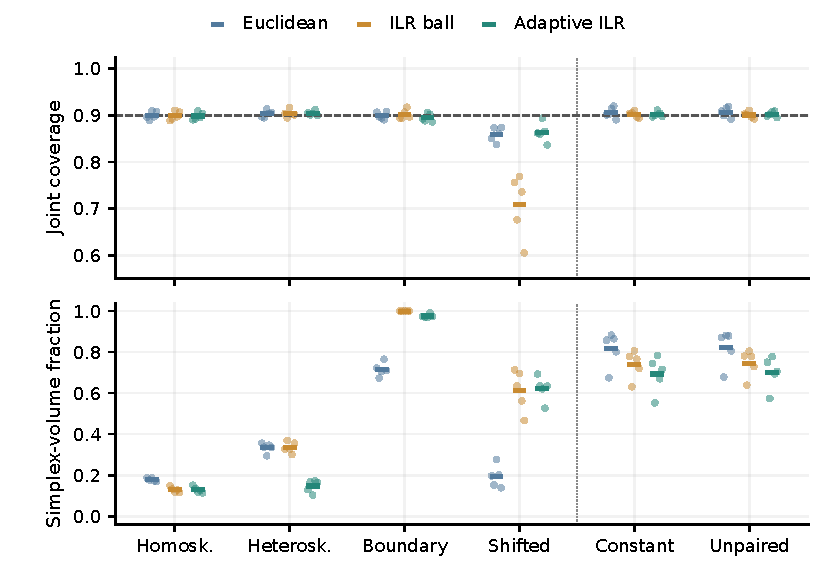
\includegraphics[width=\linewidth,trim=0 136.8 0 0,clip]{figures/coverage_volume_by_regime.pdf}
\caption{Joint response coverage.}\label{fig:coverage}
\end{subfigure}
\begin{subfigure}{\textwidth}
\centering
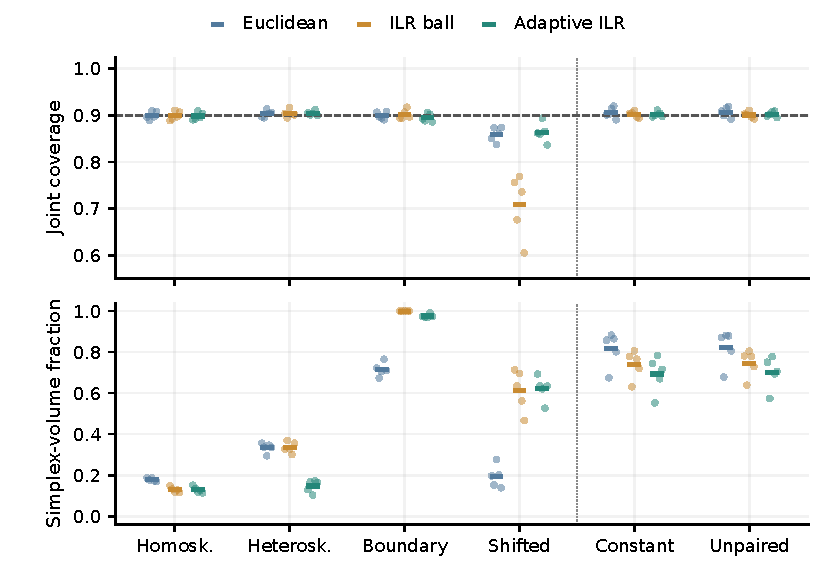
\includegraphics[width=\linewidth,trim=0 0 0 136.8,clip]{figures/coverage_volume_by_regime.pdf}
\caption{Common-simplex volume fraction.}\label{fig:volume}
\end{subfigure}
\caption{Condition-specific coverage and common-simplex volume. Small dots are the five held-out seeds; horizontal marks are their means. The dashed line denotes nominal coverage, not a confidence bound. The dotted separator distinguishes response conditions from matched information-removal controls. Compactness and coverage must be read together: shifted Euclidean regions are smaller but under-cover, while boundary ILR regions nearly fill the simplex.}
\label{fig:comparison}
\end{figure}

\subsection{Boundary Inefficiency and Covariate-Shift Failure}
The boundary-concentrated Dirichlet condition reverses the favorable efficiency story. Adaptive ILR has volume 0.9759 and coverage 0.8947. The isotropic ILR ball has volume 0.999998, effectively the full simplex at the reported resolution, whereas the Euclidean ball uses 0.7155 with coverage 0.8992. The adaptive shape reduces volume relative to isotropic ILR but does not make the region compact relative to the raw-simplex reference. A near-full-simplex region can achieve unremarkable coverage on a boundary-concentrated response distribution because uniform simplex volume is not response probability mass. This is a limitation of the tested score/geometry combination, not an integration-based proof of good uncertainty quality.
% @evidence[[paper_data.json#final_evaluation.evaluation_evidence.episodes]]
% @evidence[[derived/summary.json]]

Under test-only covariate shift, adaptive coverage is 0.8633, below the 0.90 target. It exceeds the ILR ball's 0.7082 but is close to the Euclidean ball's 0.8592. Its volume is 0.6221, versus 0.6145 for the ILR ball and 0.1928 for Euclidean balls. The shift therefore does not yield a clean efficiency advantage: adaptive ILR is substantially larger than Euclidean while both under-cover. The known change in the test covariate law removes the premise of the ordinary calibration argument. The measurements do not isolate whether each shortfall is driven by location extrapolation, scale extrapolation, or residual-shape mismatch.
% @evidence[[paper_data.json#final_evaluation.evaluation_evidence.episodes]]
% @evidence[[derived/summary.json]]

\subsection{Local Diagnostics and Information-Removal Controls}
Figure~\ref{fig:strata} shows that marginal adaptation does not remove local imbalance. In the heteroskedastic condition, adaptive mean coverage is 0.9740 for $x_1<0$ and 0.8339 for $x_1\ge0$; the corresponding ILR-ball rates are 0.9975 and 0.8082. The adaptive score moderates this contrast but leaves substantial undercoverage in the higher-noise half. These are overlapping sign-mask summaries across seeds, not independent partitions or simultaneous conditional confidence statements. No evaluated boundary-tertile coverage guarantee can be inferred from them.
% @evidence[[paper_data.json#final_evaluation.evaluation_evidence.episodes]]

\begin{figure}[t]
\centering
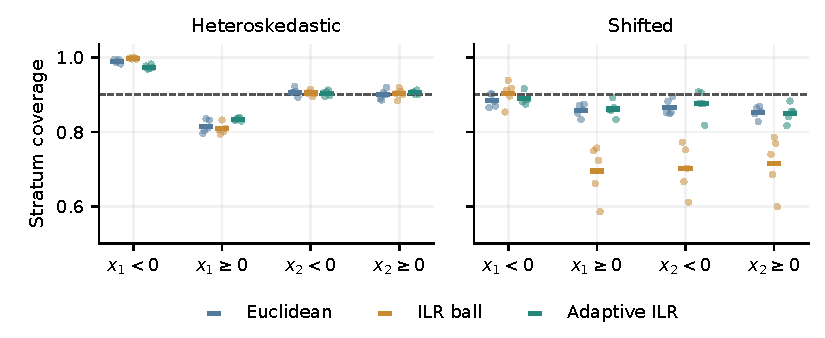
\includegraphics[width=\textwidth]{figures/descriptive_sign_strata.pdf}
\caption{Descriptive sign-stratum reliability in heteroskedastic and shifted conditions. Dots show each held-out seed and bars show means. Masks for different covariates overlap; their coverage rates are not simultaneous guarantees. The nominal line is a reference only. No empty-mask zero encodings are plotted.}
\label{fig:strata}
\end{figure}

Removing informative covariates produces wide adaptive regions: mean volume is 0.6932 for constant inputs and 0.7004 after training-pair derangement, compared with 0.1476 in the intact heteroskedastic condition. Their adaptive coverage remains approximately nominal at 0.9019 and 0.9023. This shows the efficiency contrast depends on accessible training information; it does not certify any particular information-extraction mechanism. The constant-input case also exposes a reporting artifact. The retained worst-stratum summary is 0.0 because empty negative-sign masks are encoded as zero. It is not an observed subgroup with zero coverage. We preserve the original summary and its limitation rather than silently substituting a different statistic; per-mask counts are not retained in the episode records.
% @evidence[[paper_data.json#final.metric.worst_stratum_coverage]]
% @evidence[[paper_data.json#final_evaluation.evaluation_evidence.episodes]]
% @evidence[[source_evidence/evaluate_final.py#L924-L928]]

\subsection{Aggregate Comparisons and Completed Checks}
The equal-weight six-condition adaptive averages are coverage 0.8942 and volume 0.5446. Aggregate paired contrasts in Table~\ref{tab:contrasts} favor adaptive ILR over the isotropic ILR reference in both coverage and volume, but not over Euclidean in volume. In particular, the Euclidean volume-reduction interval is entirely negative. This aggregate includes correlated C2-derived controls and the shifted condition, so it is not a population marginal coverage estimate or an estimate over six independent task families. The separate condition results, rather than this summary, establish the paper's central trade-off.
% @evidence[[paper_data.json#final.metric.marginal_coverage]]
% @evidence[[paper_data.json#final.metric.normalized_volume]]
% @evidence[[paper_data.json#final_evaluation.evaluation_evidence.episodes]]

\begin{table}[t]
\centering\small
\begin{tabular}{llrr}
\toprule
Comparator & Contrast & Mean & Paired bootstrap 95\% \\
\midrule
Euclidean & Coverage: adaptive minus reference & $-0.0014$ & $[-0.0065,0.0039]$ \\
Euclidean & Volume: reference minus adaptive & $-0.0346$ & $[-0.0546,-0.0115]$ \\
ILR ball & Coverage: adaptive minus reference & $0.0251$ & $[0.0185,0.0319]$ \\
ILR ball & Volume: reference minus adaptive & $0.0496$ & $[0.0306,0.0618]$ \\
\bottomrule
\end{tabular}
\caption{Equal-weight contrasts across all six conditions. Positive values favor adaptive ILR. Intervals resample five paired seed blocks and retain all conditions together; few-seed percentile intervals are unstable and not multiplicity-adjusted. They are not per-condition error bars.}
\label{tab:contrasts}
% @evidence[[paper_data.json#final.metric.coverage_gap_vs_euclidean]]
% @evidence[[paper_data.json#final.metric.volume_gain_vs_euclidean]]
% @evidence[[paper_data.json#final.metric.coverage_gap_vs_ilr]]
% @evidence[[paper_data.json#final.metric.volume_gain_vs_ilr]]
% @evidence[[paper_data.json#final_evaluation.evaluation_evidence.episodes]]
\end{table}

The final evaluation completed and satisfied its recorded qualification checks. Observed checks include query-order/subset invariance, singleton/full-simplex membership controls, matched interventions, and a replay. Their scope is operational: they do not establish conditional validity, shift robustness, a comprehensive nonadaptivity audit, or universal superiority. No unreported diagnostic is inferred from the qualification outcome. The performance failures above remain scientific limitations notwithstanding completion of these checks.
% @evidence[[paper_data.json#grounding_sources.final.qualification.status]]
% @evidence[[paper_data.json#grounding_sources.final.qualification.outcome]]
% @evidence[[paper_data.json#grounding_sources.final.qualification.correct]]
% @evidence[[paper_data.json#final_evaluation.evaluation_evidence.episodes]]

\section{Discussion and Limitations}
The information-removal controls help interpret compactness without establishing a mechanism. With constant covariates, a fitted region cannot distinguish test locations from their inputs, so a wide region reflects the heterogeneous response distribution left after removing that information. With deranged training pairs, the calibration/test association is unchanged but the fitted relationship is degraded. Independent calibration can still adjust a frozen score to the resulting marginal residual distribution. Neither control is equivalent to testing whether the intact model has recovered a particular conditional law. In particular, their near-nominal marginal coverage does not validate the intact model's local reliability. The useful contrast is the loss of compactness when predictive training information is removed, not a proof that every adaptive shape factor is necessary.
% @evidence[[source_evidence/evaluate_final.py#L1007-L1036]]
% @evidence[[paper_data.json#final_evaluation.evaluation_evidence.episodes]]

The study separates two questions often collapsed into a single claim of reliable uncertainty. Independent calibration governs a marginal rank statement under a specified sampling law; geometry governs which compositions are included at a given calibrated threshold. An adaptive score can improve measured efficiency without improving every local coverage rate. Conversely, a large region can have poor coverage after a distribution change. These are different failures and require different evidence. Here the shifted law is documented, but attribution to a specific fitting component remains unresolved.

The common volume measure is useful precisely because it is coordinate-independent across the evaluated methods, not because it is the only appropriate utility. Uniform simplex volume puts weight on different locations than a boundary-concentrated response distribution. Consequently, near-unit volume does not imply near-unit response coverage. Application-specific costs, alternative base measures, or calibrated probability-forecast scores could change the practical ranking; they were not measured. The retained scalar objective should therefore not be interpreted as a proper probabilistic score or as a replacement for joint coverage and set size \citep{Gneiting2007}.

Several limitations constrain interpretation. The response families are synthetic, strictly positive, and low-dimensional relative to many applications. No real dataset, structural-zero case, label-set task, alternative score geometry, or weighted shift calibration was evaluated. The boundary and shifted conditions also change response family and dimension relative to the logistic-normal conditions; their comparison is a regime contrast, not an isolated intervention on boundary proximity or shift. The reference fits use fewer training rows than the adaptive location, and the auxiliary residual comparison bundles changes. Neither causal mechanism attribution nor an optimality claim follows.
% @evidence[[source_evidence/evaluate_final.py#L776-L814]]
% @evidence[[source_evidence/evaluate_final.py#L665-L672]]
% @evidence[[paper_data.json#all_programs]]

Only five held-out seed blocks are available, and their shared response/control structure limits the information in an aggregate interval. The frozen evaluation reduces direct reuse of development measurements; it is not a broad certification against all adaptive reuse. Exact reproduction also requires the stored resource arrays: their generator uses private entropy, so the published seed labels alone cannot recreate them. We provide readable evaluated source copies, resource manifests, complete retained numerical summaries, and deterministic figure/table construction. This supports inspection and replay using the distributed arrays, while explicitly preserving the limits of regeneration and of the evidence itself.
% @evidence[[source_evidence/final_resource_manifest.json]]
% @evidence[[source_evidence/evaluate_final.py#L768-L814]]
% @evidence[[derived/complete_results.json]]

\section{Conclusion}
Training-adaptive ILR ellipsoids offer a favorable measured coverage--volume trade-off for the evaluated heteroskedastic logistic-normal responses, but that finding does not transfer uniformly across the simplex-valued conditions. The same configuration nearly fills the simplex for boundary-concentrated Dirichlet responses and remains below nominal coverage under covariate shift. Even the favorable condition retains pronounced sign-stratum imbalance. These limitations are part of the main result, not exceptions removed from the evaluation.

The methodological lesson is to compare geometries on the same response-space measure and to separate uncertainty sources. Calibration, finite-test coverage, integration precision, and seed-to-seed variability answer different questions. The present evidence supports a narrowly scoped empirical comparison of complete fitted systems, with independent calibration and explicit failure analysis; it does not establish a uniquely effective component, conditional validity, real-data generalization, or robustness to unmeasured shifts.
% @evidence[[paper_data.json#final_evaluation.evaluation_evidence.episodes]]

\clearpage
\bibliography{references}
\bibliographystyle{paper}
\clearpage
\appendix
\section{Supplementary Information}
\subsection{Exact Residual Geometry and Numerical Safeguards}
The inspected implementation is reproduced in \path{source_evidence/adaptive.py}; the source inventory maps each copy to its evaluated location and SHA256. Features are formed at lines 78--85, training fits at lines 103--131, and row-wise factors at lines 190--198. The quadratic design has 21 columns: an intercept, five linear terms, five squares, and ten cross-products. With design matrix $\Phi$, every ridge fit has the explicit form $(\Phi^T\Phi+\lambda I)^{-1}\Phi^TZ$, implemented through a linear solve. The location penalty is $0.01$; the log-residual-square penalty is $5$. The residual offset, variance-prediction clipping, and standardized-residual clipping are exactly those in equations~\eqref{eq:scale}--\eqref{eq:shape}. No test response enters these fits.
% @evidence[[source_evidence/adaptive.py#L78-L131]]

The contrast basis in \path{source_evidence/evaluate_final.py}, lines 624--630, has column $j$ proportional to $(1,\ldots,1,-j,0,\ldots,0)$, normalized by $\sqrt{j(j+1)}$, for $j=1,\ldots,K-1$. Thus ILR coordinates span the sum-zero log-contrast space. Predicted boundary scores use the inverse-ILR location, not observed test responses. Both calibration and future queries use the same right-sided group routing. With fewer than four training rows, the implementation falls back to a full-data location, zero log-variance coefficients, and identity group factors; the released full-size evaluations do not exercise that branch. Empty training groups still receive the pooled positive shape through shrinkage. This operational fallback is distinct from the empty evaluation masks discussed below.
% @evidence[[source_evidence/evaluate_final.py#L624-L637]]
% @evidence[[source_evidence/adaptive.py#L90-L131]]

The inverse transform maps a Euclidean ellipsoid in ILR space to a generally nonellipsoidal region in raw coordinates. The study consequently calls it an ILR ellipsoid and evaluates membership after the appropriate transform. Neither its ILR determinant nor a product of coordinate widths equals its raw-simplex volume fraction. Our volume comparisons use direct membership integration, avoiding a change-of-variables approximation.
% @evidence[[source_evidence/evaluate_final.py#L882-L938]]

\subsection{Synthetic Generators and Matched Interventions}\label{sec:generators}
Each stored resource has covariates $X_i\sim N(0,I_5)$ before any test intervention. A seed-specific coefficient matrix has independent $N(0,0.35^2)$ entries, and the ILR mean is $\mu(x)=x^TW+0.2x_1^2\mathbf1$. For C1 and C2, the observed ILR response is $\mu(x)+\sigma(x)\odot\epsilon$ with independent standard-normal $\epsilon$. C1 has constant coordinate scales $0.35$; C2 multiplies those scales by $\exp\{0.65\clip(x_1,-3,3)\}$ and a linear sequence from $0.5$ to $1.5$. These are data-generator parameters, not fitted hyperparameters.
% @evidence[[source_evidence/evaluate_final.py#L776-L795]]

For C3, add $2.3$ to the first coordinate of $\mu$ and compute $p=h(\mu)$. Generate independent gamma variables with shapes $a_j=\max(3p_j,0.15)$ and normalize them. For C4, use $a_j=\max(14p_j,0.15)$ with no such mean offset; only its test covariates receive the stated shift/rescaling. The component floor means that the actual mean is proportional to $a$, not necessarily exactly $p$. Nonpositive or nonfinite gamma draws are redrawn, for at most 16 passes, and any unresolved draw fails resource construction. This produces strictly positive compositions, not a structural-zero model. C5 and C6 are derived from stored C2 arrays exactly as described in the main text, rather than independently generated synthetic samples.
% @evidence[[source_evidence/evaluate_final.py#L795-L814]]
% @evidence[[source_evidence/evaluate_final.py#L1007-L1036]]

The resource manifest records training rows $[0,4096)$, calibration rows $[4096,6144)$, and test rows $[6144,9984)$, together with per-file hashes. Parameter, covariate, response, and volume-probe random substreams are derived from stored private entropy. The arrays and manifest, not the integer labels alone, define the evaluated datasets. The experiment is entirely synthetic and requires no external dataset account or license acceptance.
% @evidence[[source_evidence/final_resource_manifest.json]]

\subsection{Complete Coverage and Common-Volume Measurements}
The following table contains all final seed--condition measurements for the three methods. Means in the main text are unweighted arithmetic averages of the five corresponding rows. \path{derived/complete_results.json} additionally preserves every per-anchor volume fraction, all sign-mask rates, calibrated radii and ranks, point errors, and paired integration standard errors. It also labels the empty-mask positions without replacing the original rates. The original individual membership indicators remain in \path{paper_data.json}. No uncertainty interval in this supplement is a simultaneous conditional-coverage guarantee.
% @evidence[[derived/complete_results.json]]
% @evidence[[paper_data.json#final_evaluation.evaluation_evidence.episodes]]
{\footnotesize\setlength{\tabcolsep}{3pt}% BEGIN GENERATED SEED RESULTS
% @evidence[[paper_data.json#final_evaluation.evaluation_evidence.episodes]]
\begin{longtable}{rrlrrrr}
\caption{Complete held-out seed-level measurements. Coverage intervals are Wilson intervals; volume SE is conditional Monte Carlo integration error, not between-seed variability.}\\
\toprule
Seed & Case & Method & Coverage & Wilson 95\% & Volume & MC SE \\
\midrule\endfirsthead
\toprule Seed & Case & Method & Coverage & Wilson 95\% & Volume & MC SE \\ \midrule\endhead
1009 & C1 & Euclidean & 0.8961 & [0.8860,0.9054] & 0.1873 & 0.00076 \\
1009 & C1 & ILR ball & 0.8885 & [0.8782,0.8981] & 0.1492 & 0.00069 \\
1009 & C1 & Adaptive ILR & 0.8904 & [0.8801,0.8999] & 0.1513 & 0.00069 \\
1009 & C2 & Euclidean & 0.8969 & [0.8869,0.9061] & 0.3560 & 0.00092 \\
1009 & C2 & ILR ball & 0.9036 & [0.8939,0.9126] & 0.3276 & 0.00089 \\
1009 & C2 & Adaptive ILR & 0.9052 & [0.8955,0.9141] & 0.1301 & 0.00063 \\
1009 & C3 & Euclidean & 0.9065 & [0.8969,0.9153] & 0.7226 & 0.00069 \\
1009 & C3 & ILR ball & 0.8940 & [0.8839,0.9034] & 1.0000 & 0.00000 \\
1009 & C3 & Adaptive ILR & 0.8919 & [0.8817,0.9014] & 0.9743 & 0.00030 \\
1009 & C4 & Euclidean & 0.8505 & [0.8389,0.8614] & 0.1970 & 0.00071 \\
1009 & C4 & ILR ball & 0.7557 & [0.7419,0.7691] & 0.7136 & 0.00045 \\
1009 & C4 & Adaptive ILR & 0.8617 & [0.8504,0.8723] & 0.6930 & 0.00075 \\
1009 & C5 & Euclidean & 0.9010 & [0.8912,0.9101] & 0.8578 & 0.00068 \\
1009 & C5 & ILR ball & 0.9042 & [0.8944,0.9131] & 0.7782 & 0.00081 \\
1009 & C5 & Adaptive ILR & 0.8969 & [0.8869,0.9061] & 0.7439 & 0.00085 \\
1009 & C6 & Euclidean & 0.9086 & [0.8991,0.9173] & 0.8711 & 0.00065 \\
1009 & C6 & ILR ball & 0.9023 & [0.8925,0.9113] & 0.7805 & 0.00081 \\
1009 & C6 & Adaptive ILR & 0.8982 & [0.8882,0.9073] & 0.7505 & 0.00084 \\
2027 & C1 & Euclidean & 0.8893 & [0.8790,0.8989] & 0.1763 & 0.00074 \\
2027 & C1 & ILR ball & 0.8924 & [0.8823,0.9019] & 0.1328 & 0.00065 \\
2027 & C1 & Adaptive ILR & 0.8924 & [0.8823,0.9019] & 0.1340 & 0.00066 \\
2027 & C2 & Euclidean & 0.8948 & [0.8847,0.9041] & 0.3362 & 0.00092 \\
2027 & C2 & ILR ball & 0.8945 & [0.8844,0.9039] & 0.3687 & 0.00093 \\
2027 & C2 & Adaptive ILR & 0.9010 & [0.8912,0.9101] & 0.1679 & 0.00070 \\
2027 & C3 & Euclidean & 0.8969 & [0.8869,0.9061] & 0.6733 & 0.00068 \\
2027 & C3 & ILR ball & 0.8940 & [0.8839,0.9034] & 1.0000 & 0.00000 \\
2027 & C3 & Adaptive ILR & 0.8883 & [0.8779,0.8979] & 0.9707 & 0.00031 \\
2027 & C4 & Euclidean & 0.8732 & [0.8623,0.8833] & 0.1520 & 0.00064 \\
2027 & C4 & ILR ball & 0.6758 & [0.6608,0.6904] & 0.6346 & 0.00060 \\
2027 & C4 & Adaptive ILR & 0.8591 & [0.8478,0.8698] & 0.6367 & 0.00079 \\
2027 & C5 & Euclidean & 0.9018 & [0.8920,0.9108] & 0.6749 & 0.00091 \\
2027 & C5 & ILR ball & 0.9052 & [0.8955,0.9141] & 0.6313 & 0.00094 \\
2027 & C5 & Adaptive ILR & 0.8997 & [0.8898,0.9088] & 0.5525 & 0.00097 \\
2027 & C6 & Euclidean & 0.8992 & [0.8893,0.9083] & 0.6785 & 0.00091 \\
2027 & C6 & ILR ball & 0.9016 & [0.8917,0.9106] & 0.6383 & 0.00094 \\
2027 & C6 & Adaptive ILR & 0.9013 & [0.8915,0.9103] & 0.5740 & 0.00096 \\
3049 & C1 & Euclidean & 0.9096 & [0.9002,0.9183] & 0.1866 & 0.00076 \\
3049 & C1 & ILR ball & 0.9107 & [0.9012,0.9193] & 0.1176 & 0.00062 \\
3049 & C1 & Adaptive ILR & 0.9094 & [0.8999,0.9181] & 0.1173 & 0.00062 \\
3049 & C2 & Euclidean & 0.9138 & [0.9045,0.9223] & 0.2947 & 0.00088 \\
3049 & C2 & ILR ball & 0.9167 & [0.9075,0.9250] & 0.3271 & 0.00089 \\
3049 & C2 & Adaptive ILR & 0.9042 & [0.8944,0.9131] & 0.1027 & 0.00058 \\
3049 & C3 & Euclidean & 0.8943 & [0.8841,0.9036] & 0.7056 & 0.00069 \\
3049 & C3 & ILR ball & 0.9065 & [0.8969,0.9153] & 1.0000 & 0.00000 \\
3049 & C3 & Adaptive ILR & 0.9060 & [0.8963,0.9148] & 0.9684 & 0.00022 \\
3049 & C4 & Euclidean & 0.8378 & [0.8258,0.8491] & 0.2754 & 0.00082 \\
3049 & C4 & ILR ball & 0.7688 & [0.7551,0.7818] & 0.6959 & 0.00054 \\
3049 & C4 & Adaptive ILR & 0.8938 & [0.8836,0.9031] & 0.6202 & 0.00085 \\
3049 & C5 & Euclidean & 0.9141 & [0.9048,0.9225] & 0.8837 & 0.00063 \\
3049 & C5 & ILR ball & 0.9102 & [0.9007,0.9188] & 0.8066 & 0.00077 \\
3049 & C5 & Adaptive ILR & 0.9112 & [0.9018,0.9198] & 0.7835 & 0.00080 \\
3049 & C6 & Euclidean & 0.9156 & [0.9064,0.9240] & 0.8813 & 0.00063 \\
3049 & C6 & ILR ball & 0.9104 & [0.9010,0.9190] & 0.8048 & 0.00077 \\
3049 & C6 & Adaptive ILR & 0.9081 & [0.8985,0.9168] & 0.7784 & 0.00081 \\
4051 & C1 & Euclidean & 0.8969 & [0.8869,0.9061] & 0.1720 & 0.00073 \\
4051 & C1 & ILR ball & 0.8969 & [0.8869,0.9061] & 0.1277 & 0.00064 \\
4051 & C1 & Adaptive ILR & 0.8956 & [0.8855,0.9049] & 0.1260 & 0.00064 \\
4051 & C2 & Euclidean & 0.9039 & [0.8942,0.9128] & 0.3462 & 0.00092 \\
4051 & C2 & ILR ball & 0.9013 & [0.8915,0.9103] & 0.3002 & 0.00087 \\
4051 & C2 & Adaptive ILR & 0.9122 & [0.9029,0.9208] & 0.1725 & 0.00068 \\
4051 & C3 & Euclidean & 0.8901 & [0.8798,0.8996] & 0.7653 & 0.00066 \\
4051 & C3 & ILR ball & 0.9174 & [0.9083,0.9257] & 1.0000 & 0.00000 \\
4051 & C3 & Adaptive ILR & 0.9018 & [0.8920,0.9108] & 0.9915 & 0.00018 \\
4051 & C4 & Euclidean & 0.8607 & [0.8494,0.8713] & 0.2011 & 0.00071 \\
4051 & C4 & ILR ball & 0.7357 & [0.7215,0.7494] & 0.5620 & 0.00056 \\
4051 & C4 & Adaptive ILR & 0.8656 & [0.8545,0.8760] & 0.5261 & 0.00087 \\
4051 & C5 & Euclidean & 0.9198 & [0.9108,0.9280] & 0.8648 & 0.00067 \\
4051 & C5 & ILR ball & 0.8958 & [0.8858,0.9051] & 0.7654 & 0.00083 \\
4051 & C5 & Adaptive ILR & 0.9042 & [0.8944,0.9131] & 0.6702 & 0.00092 \\
4051 & C6 & Euclidean & 0.9185 & [0.9094,0.9267] & 0.8792 & 0.00064 \\
4051 & C6 & ILR ball & 0.8961 & [0.8860,0.9054] & 0.7788 & 0.00081 \\
4051 & C6 & Adaptive ILR & 0.9089 & [0.8993,0.9176] & 0.6935 & 0.00090 \\
5059 & C1 & Euclidean & 0.9083 & [0.8988,0.9171] & 0.1686 & 0.00072 \\
5059 & C1 & ILR ball & 0.9070 & [0.8974,0.9158] & 0.1149 & 0.00061 \\
5059 & C1 & Adaptive ILR & 0.9039 & [0.8942,0.9128] & 0.1142 & 0.00061 \\
5059 & C2 & Euclidean & 0.9057 & [0.8961,0.9146] & 0.3350 & 0.00092 \\
5059 & C2 & ILR ball & 0.9010 & [0.8912,0.9101] & 0.3558 & 0.00092 \\
5059 & C2 & Adaptive ILR & 0.8992 & [0.8893,0.9083] & 0.1647 & 0.00070 \\
5059 & C3 & Euclidean & 0.9081 & [0.8985,0.9168] & 0.7107 & 0.00068 \\
5059 & C3 & ILR ball & 0.8961 & [0.8860,0.9054] & 1.0000 & 0.00001 \\
5059 & C3 & Adaptive ILR & 0.8857 & [0.8752,0.8954] & 0.9743 & 0.00031 \\
5059 & C4 & Euclidean & 0.8740 & [0.8631,0.8841] & 0.1386 & 0.00061 \\
5059 & C4 & ILR ball & 0.6049 & [0.5894,0.6203] & 0.4662 & 0.00057 \\
5059 & C4 & Adaptive ILR & 0.8362 & [0.8242,0.8476] & 0.6347 & 0.00080 \\
5059 & C5 & Euclidean & 0.8904 & [0.8801,0.8999] & 0.8018 & 0.00078 \\
5059 & C5 & ILR ball & 0.8935 & [0.8833,0.9029] & 0.7201 & 0.00088 \\
5059 & C5 & Adaptive ILR & 0.8977 & [0.8877,0.9068] & 0.7158 & 0.00088 \\
5059 & C6 & Euclidean & 0.8917 & [0.8814,0.9011] & 0.8058 & 0.00077 \\
5059 & C6 & ILR ball & 0.8922 & [0.8820,0.9016] & 0.7288 & 0.00087 \\
5059 & C6 & Adaptive ILR & 0.8951 & [0.8850,0.9044] & 0.7057 & 0.00089 \\
\bottomrule
\end{longtable}
% END GENERATED SEED RESULTS}

\subsection{Auxiliary Training-Configuration Comparisons}
The development corpus has seeds 101, 211, and 307, with 2048 training, 1024 calibration, and 2048 test rows. Figure~\ref{fig:aux} compares three adaptive configurations directly on those common data. The single-split configuration estimates locations from the first three quarters of training rows and fits scale and shape from the remaining residuals. The four-fold configuration uses held-out residuals from all training rows and refits its location using all rows. Thus residual estimation, allocation, and final location fitting change together. No isolated full-data-refit or residual-fold-count experiment is available. These development measurements do not provide independent held-out evidence for the two auxiliary configurations.
% @evidence[[source_evidence/search_resource_manifest.json]]
% @evidence[[paper_data.json#all_programs]]
% @evidence[[source_evidence/single_split.py#L108-L131]]
% @evidence[[source_evidence/adaptive.py#L108-L131]]

The interpolated configuration retains four-fold residual fitting and the same shape regularization, but freezes boundary-score anchors at training quantiles $1/6,1/2,5/6$. Duplicate anchors are merged by averaging their shape matrices. Between distinct anchors it convexly interpolates the covariance-shaped matrices, with endpoint clamping, and takes a Cholesky factor after interpolation. This contrasts with hard group routing. The measured differences do not establish a consistent advantage from interpolation. No shrinkage sweep, Hellinger-score comparison, groupwise calibration, or alternative compositional transform is present in the released results.
% @evidence[[source_evidence/interpolated.py#L121-L151]]
% @evidence[[source_evidence/interpolated.py#L210-L240]]
% @evidence[[derived/search_comparison.json]]

\begin{figure}[ht]
\centering
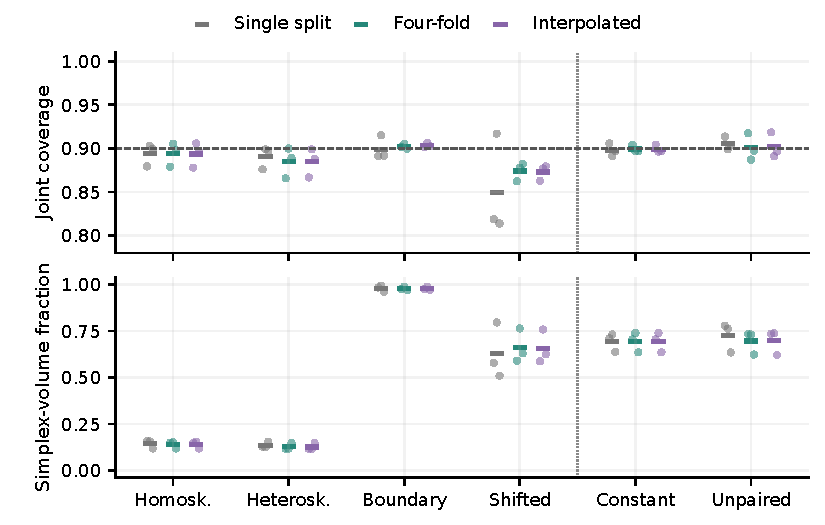
\includegraphics[width=\textwidth]{figures/search_configuration_comparison.pdf}
\caption{Auxiliary development-data comparisons, not final replications. Dots denote three shared seeds and bars their means. The four-fold versus single-split contrast bundles residual estimation and location/data-allocation changes. Continuous interpolation alters the covariance routing but has no established consistent benefit. These comparisons do not identify a uniquely effective component.}
\label{fig:aux}
\end{figure}

\subsection{Uncertainty Estimands and Operational Checks}
For a fitted/calibrated region, the test indicator average estimates response coverage under the condition's test law; a Wilson interval quantifies its finite-test binomial uncertainty. It does not quantify variation from resampling training or calibration data. Conditional on fixed anchors and fitted regions, the volume integration standard error is
\begin{equation}
 \widehat{\mathrm{SE}}_{\mathrm{MC}}(\widehat V)
 =\frac1A\sqrt{\sum_{a=1}^A\frac{\widehat p_a(1-\widehat p_a)}{M}}.
\end{equation}
The paired volume error uses the sample variance of shared-probe membership differences at each anchor, summed across anchors and divided by $A^2$. This exploits pairing without treating membership outcomes of different methods as independent. Neither error includes anchor-selection variability. Seed dispersion and the paired bootstrap address a different source of uncertainty. The retained bootstrap uses random seed 80801, resamples five seed blocks 2000 times, and preserves all within-seed case dependence; this is a small empirical resampling distribution, not a broad generalization guarantee.
% @evidence[[source_evidence/evaluate_final.py#L907-L938]]
% @evidence[[source_evidence/evaluate_final.py#L1220-L1229]]
% @evidence[[source_evidence/evaluate_final.py#L1266-L1294]]

Empty negative-sign masks arise deterministically for the constant-input condition because all queried covariates equal zero. The evaluator encodes their coverage as $0.0$ and subsequently takes a minimum over seed-averaged stratum rates. The registered worst-stratum statistic is therefore $0.0$ for an empty-mask reason. Its denominator is not a nonempty subgroup, and it must not be interpreted as zero conditional response coverage. Episode records do not retain per-mask counts, so this manuscript does not construct count-weighted or nonempty-mask replacement summaries.
% @evidence[[source_evidence/evaluate_final.py#L924-L928]]
% @evidence[[source_evidence/evaluate_final.py#L1254-L1263]]
% @evidence[[paper_data.json#final.metric.worst_stratum_coverage]]

\begin{table}[ht]
\centering\small
\begin{tabular}{p{.29\textwidth}p{.63\textwidth}}
\toprule
Observed check & What the retained evidence supports \\
\midrule
Singleton and full simplex & Membership controls give respectively coverage/volume $0/0$ and $1/1$ on the continuous test/probe samples. \\
Query invariance & Reordered and subset predictions agree with corresponding fixed-fit outputs within the evaluator tolerances. \\
Matched interventions & Covariates are actually zeroed for C5; the C6 cyclic training permutation has no fixed row. \\
Replay & The retained replay is complete. It is not an exhaustive reproducibility or adaptivity audit. \\
Final qualification & The evaluation is completed and qualified, independently of the observed coverage and volume limitations. \\
\bottomrule
\end{tabular}
\caption{Operational checks and their limited interpretation. No unavailable diagnostic or reason for a hypothetical failure is inferred.}
% @evidence[[paper_data.json#final_evaluation.evaluation_evidence.episodes]]
% @evidence[[paper_data.json#grounding_sources.final.qualification.outcome]]
\end{table}

The development selection criterion, retained only for reproducibility, combines each case's observed coverage $\widehat c$ and volume $\widehat V$ as $1-0.8\max(0,0.9-\widehat c)/0.9-0.2\widehat V$, followed by equal weighting across the specified cases and seeds. The final scientific comparisons report the components rather than relying on this utility. It is neither a hard coverage constraint nor evidence that all conditional targets have been met. There are three measured development configurations; none of their unavailable or unperformed component tests is treated as a measured loss.
% @evidence[[source_evidence/evaluate_final.py#L932-L938]]
% @evidence[[source_evidence/evaluate_final.py#L1245-L1263]]
% @evidence[[paper_data.json#totals]]

\subsection{Reproducibility and Evidence Provenance}
The accompanying \path{REPRODUCIBILITY.md} supplies dependency versions, source inventories, commands, and figure/table mappings. The evaluated numerical dependency is NumPy 2.2.6. Evaluation requires the Linux process-isolation facilities used by the supplied evaluator, together with the frozen NPZ corpus and its manifest. Readable evaluated implementations are bundled under \path{source_evidence/}; their inventory records original locations and hashes. Hashes identify those copies but do not replace the readable code as support for implementation claims. Figure and table reconstruction reads the released evidence registry directly and does not execute a new predictor evaluation.
% @evidence[[source_evidence/requirements.txt]]
% @evidence[[source_evidence/manifest.json]]
% @evidence[[build_artifacts.py]]

The retained per-seed evaluation durations range from 6.46 to 7.59 seconds. These are observed episode-duration totals, not end-to-end installation times or measured reproduction times on the reader's hardware. No hardware-specific runtime estimate is asserted. Dataset regeneration from public seed labels alone is not possible because the generation entropy is not encoded by those labels; exact replay depends on preserving the distributed arrays. This limitation cannot be repaired by inventing a deterministic replacement corpus.
% @evidence[[paper_data.json#final_evaluation.evaluation_evidence.episodes]]
% @evidence[[source_evidence/final_resource_manifest.json]]

References were checked by direct identifiers against bibliographic services and official abstract pages, with selected conformal full texts inspected. The supplied broad retrieval was narrowed to foundational sources relevant to the manuscript. Reading scope is recorded per reference; this is not a systematic literature review or a certification of novelty. No task-identifying literature search or citation-chain traversal was used during manuscript preparation. No prohibited-source encounter was identified in this writing step; this statement does not certify unseen earlier activity.
% @evidence[[references_provenance.json]]
% @evidence[[literature/reading_report.txt]]

\subsection{LLM Usage}
LLM agents assisted with research design proposals, implementation editing, reference-query planning, source inspection, framing, manuscript drafting, and construction of plotting and claim-mapping code. Numerical findings in this paper are retained outputs of the executable evaluation, not language-model estimates. During manuscript preparation, code derived tables and figures from those existing outputs; no new model experiment was performed. LLM-assisted evidence checking links claims to source artifacts, but does not replace scientific validation or independent review. No independent human audit is claimed.
% @evidence[[paper_data.json#all_programs]]
% @evidence[[build_artifacts.py]]

\end{document}
